\documentclass[10pt,letterpaper]{article}
\renewcommand\familydefault{\sfdefault}

\usepackage{amsmath}

\usepackage[T1]{fontenc} 
\usepackage[utf8x]{inputenc}
\usepackage[british]{babel}
\usepackage{graphicx}% Include figure files
\usepackage{blindtext} 

\usepackage{fancyvrb,xcolor}
\usepackage{upquote,textcomp}

%%% Margins
\oddsidemargin=-0.50cm
\textwidth=17.0cm
\topmargin=-2.54cm
\headheight=0cm
\headsep=2cm
\textheight=23.8cm


\usepackage{hyperref} % for urls


% Default fixed font does not support bold face
\DeclareFixedFont{\ttb}{T1}{txtt}{bx}{n}{8} % for bold
\DeclareFixedFont{\ttm}{T1}{txtt}{m}{n}{8}  % for normal

% Custom colors
\usepackage{color}
\definecolor{deepblue}{rgb}{0,0,0.5}
\definecolor{deepred}{rgb}{0.6,0,0}
\definecolor{deepgreen}{rgb}{0,0.5,0}
\definecolor{deepgray}{rgb}{0.5,0.5,0.5}

\usepackage{listings}

\lstdefinestyle{myCustomPythonStyle}{
	language=Python,
	basicstyle=\linespread{1}\small,
	otherkeywords={self},             % Add keywords here
	keywordstyle=\ttb\color{deepblue},
	emph={MyClass,__init__},          % Custom highlighting
	emphstyle=\ttm\color{deepred},    % Custom highlighting style
	commentstyle=\ttm\color{deepgray},
	stringstyle=\color{deepgreen},
	frame=tb,                         % Any extra options here
	showstringspaces=false,
	columns=fullflexible,
	keepspaces=true,
	literate={-}{-}1,				% To avoid problems with hyphen -
}


\usepackage{dirtree}



\makeatletter 
  \renewcommand\verbatim@font{\normalfont\ttfamily\color{blue}}
\makeatother

\parindent=0mm 			% Remove french indent
\setlength{\parskip}{0.3cm}


\title{ScientoPy - User Manual}


\begin{document}



\begin{center}
{\LARGE \textbf{ScientoPy v 1.3.5, Installation and User Manual\\}}
\vspace*{0.5cm}

\includegraphics[scale=0.2]{./figures/escudoUnicacuaSolo.eps}\\
\vspace*{0.5cm}
Juan Pablo Ruiz Rosero\\
\texttt{jpabloruiz@unicauca.edu.co} \\
\end{center}

\tableofcontents

\newpage

\section{Installation}

\begin{enumerate}
\item For Windows download and install the Python 3 latest version (for example Python 3.6.5) from: \\ \url{https://www.python.org/downloads/}.
\item For Debian or Ubuntu run these commands to install Python3: 
\begin{verbatim}
sudo apt-get install python3 python3-tk python3-pip
\end{verbatim}

\item To use wordCloud in Windows, install Microsoft Visual C++ Redistributable para Visual Studio 2017 according to these instructions: \url{https://www.scivision.co/python-windows-visual-c++-14-required/}

\item Install the unidecode, numpy, scipy, matplotlib, and wordcloud Python libraries. For Windows, enter in the command line (Windows + R, cmd, and Enter), and run the installation script:
\begin{verbatim}
python3 -m pip install --user unidecode numpy scipy matplotlib wordcloud
\end{verbatim}

\end{enumerate}

\section{Download the bibliometric dataset}
This section describes how to download the proper dataset from Scopus and WoS. Define a search criteria that will be used for Scopus and WoS. For this guide and for the example dataset we are using: "Internet of thing"  AND  "Gateway" 

\subsection{Download the dataset from Scopus}
\begin{enumerate}
\item Make your search with the defined search criteria for Article title, Abstract, Keywords. 
\item Select all the results and click on Export:
	\begin{center}
		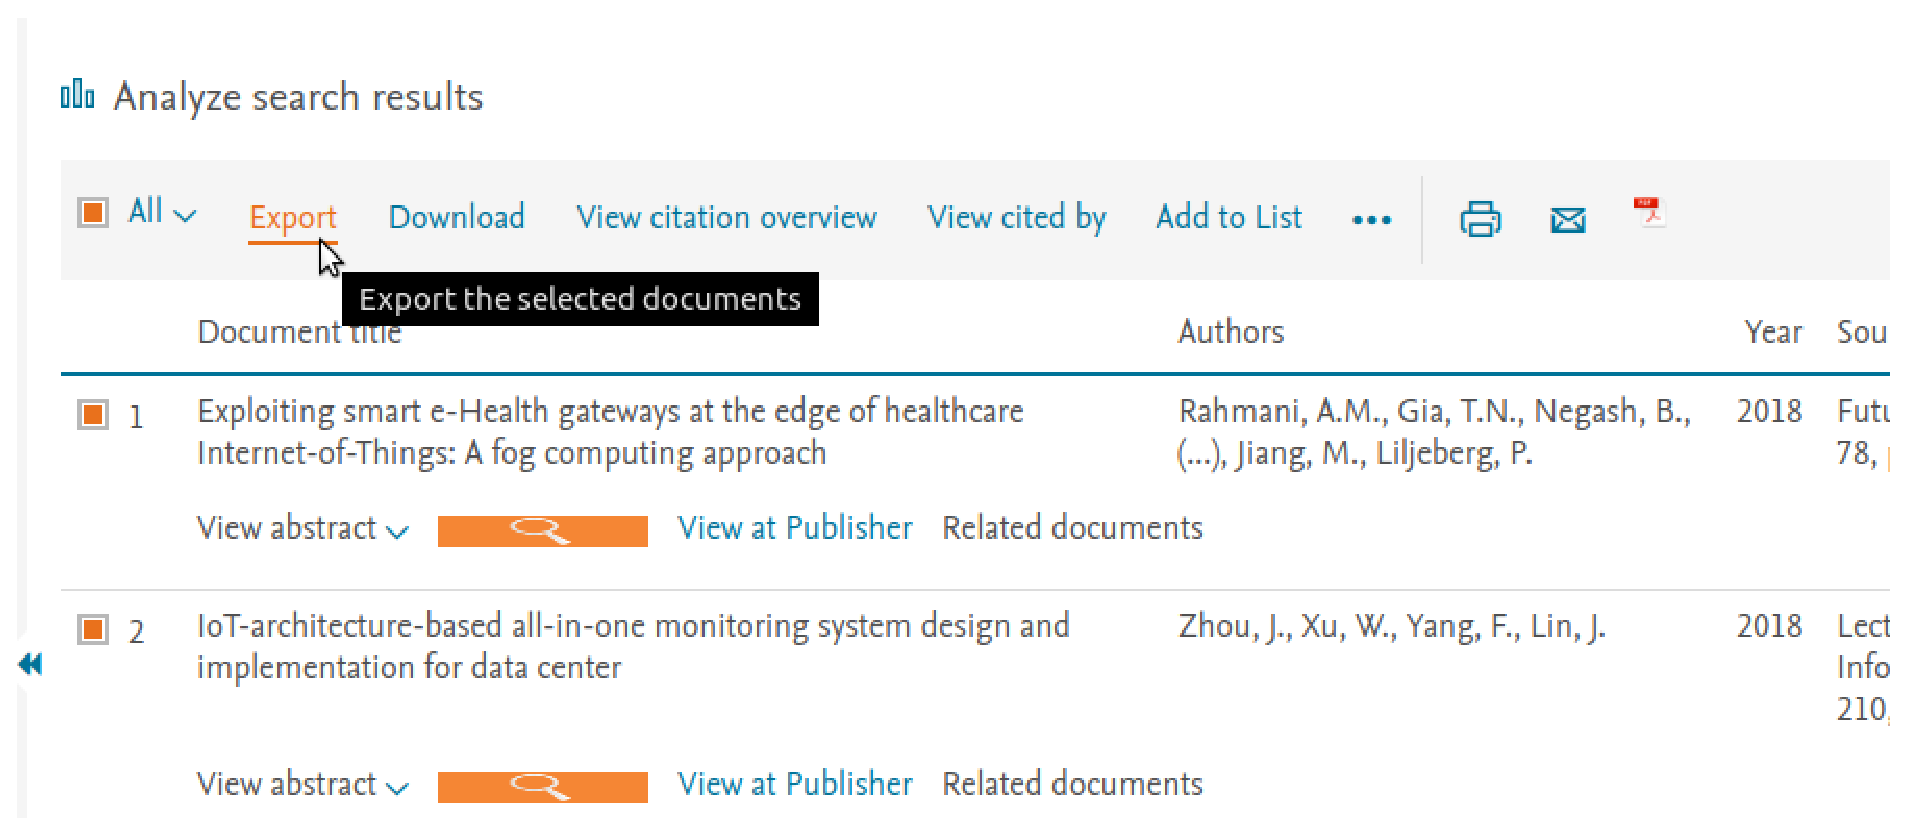
\includegraphics[scale=0.33]{./figures/scopus1.eps}
	\end{center}

\item Select as method of export \textbf{CSV (Excel)}, and select the Customize export \textbf{Citation information, Bibliographical information, Abstract and Keywords}, then click on Export: 
	\begin{center}
		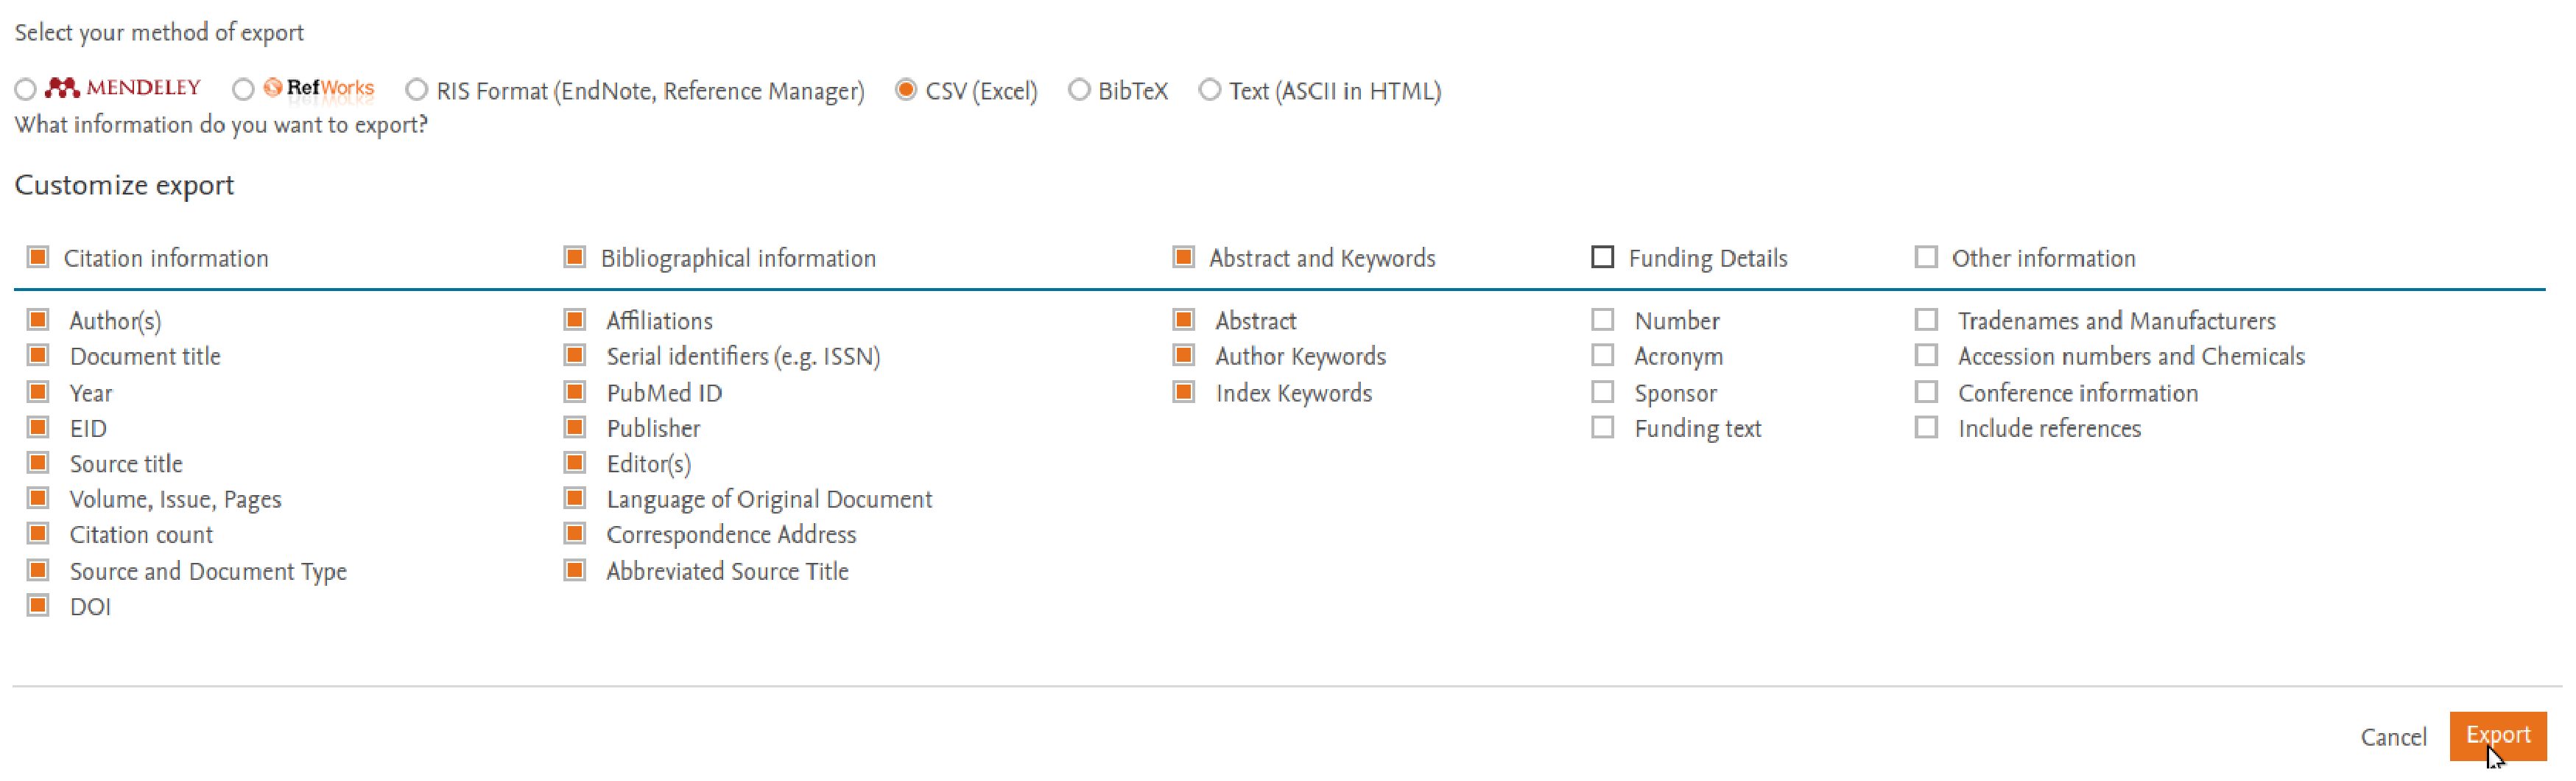
\includegraphics[scale=0.3]{./figures/scopus2.eps}
	\end{center}

\item Save the file on the folder \verb|/ScientoPy/dataIn|
\end{enumerate}


\subsection{Download the dataset from WoS}
\begin{enumerate}
\item Make your search with the defined search criteria for Topic. 
\item Select \textbf{Save in Other File Formats}
	\begin{center}
		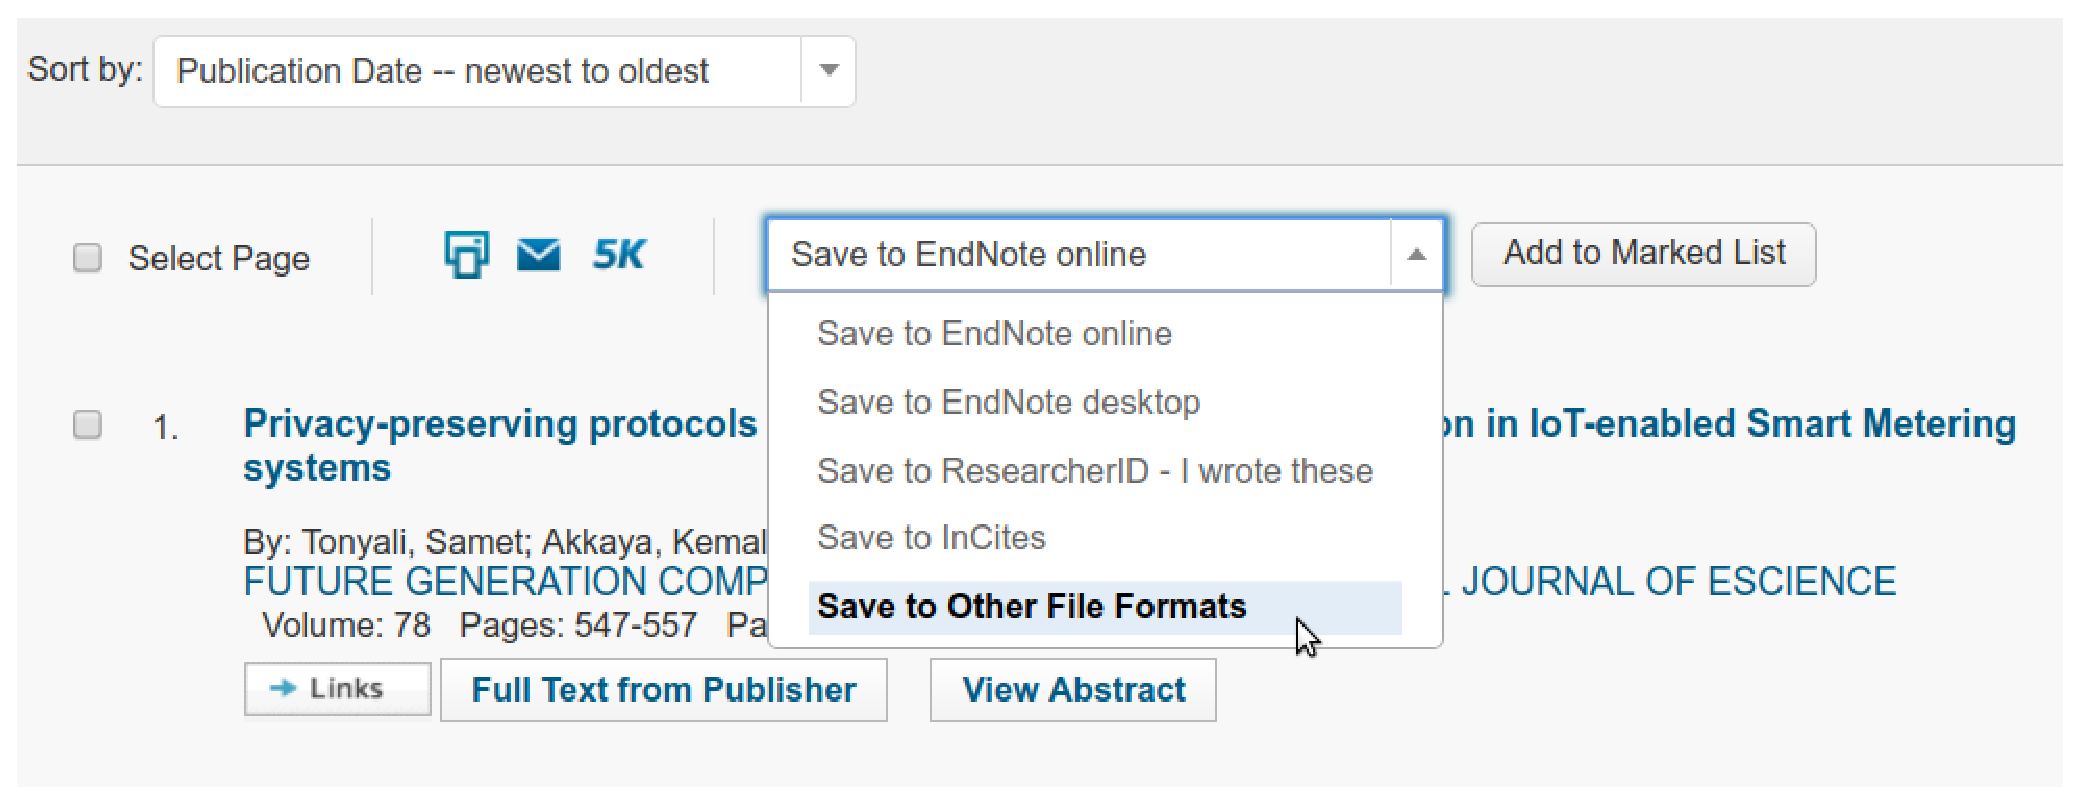
\includegraphics[scale=0.33]{./figures/wos1.eps}
	\end{center}

\item Select the number of records to download, on Record Contented select \textbf{Full Record and Cited References}, on File Format select \textbf{Tab-delimited (Win, UTF-8)}, and click on Send.
	\begin{center}
		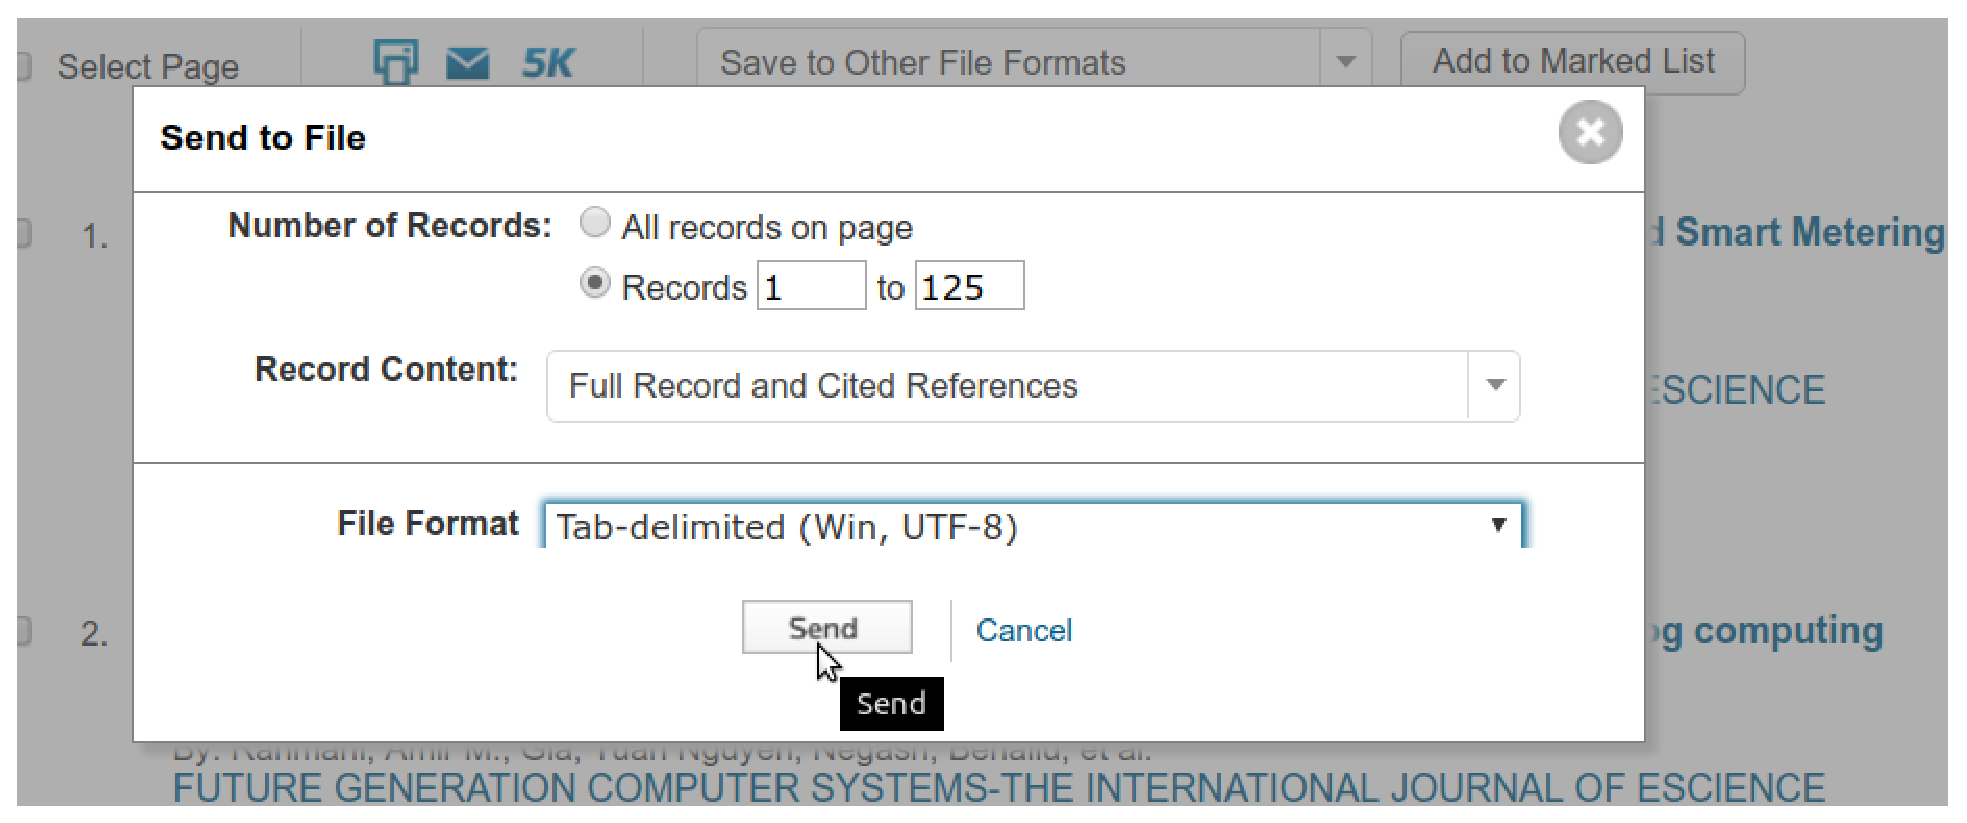
\includegraphics[scale=0.33]{./figures/wos2.eps}
	\end{center}

\item Save the file on the folder \verb|/ScientoPy/dataIn|
\end{enumerate}

\section{Running the ScientoPy scripts}

This section describes the ScientoPy scripts to preprocess and analyze the bibliometric dataset. 

\subsection{Preprocessing}

First we need to preprocess the downloaded dataset. This preprocess merge all the downloaded files from one folder to a single file. Also, this process remove the duplicated files. To preprocess the example dataset ("Internet of thing"  AND  "Gateway" located in dataInExample) run this command inside ScientoPy folder: 
\begin{verbatim}
python3 preProcess.py dataInExample
\end{verbatim}

Then, inside the folder \verb|ScientoPy/dataPre| you will find the following files: 
\begin{itemize}
\item \textbf{papersPreprocessed.tsv:} this file contains the information of all papers after the pre-process. This file will be used by the others scripts as the input data. 
\item \textbf{PreprocessedBrief.tsv:} this file briefs the pre-process statics results, such as duplicated papers removed, types of documents, and others. 
\end{itemize}

To find more options of the preprocessing script you can run:
\begin{verbatim}
python3 preProcess.py -h
\end{verbatim}

\subsection{Extract the top topics}

With this script you can extract the top topics of a selected criterion. The ScientoPy criterion are described on Table \ref{table_criterion}:

\begin{table}[h]
	\centering
	\caption{ScientoPy criterion description}
	\label{table_criterion}
	
	\renewcommand{\arraystretch}{1.5}
	\begin{tabular}{p{3.5cm} p{10cm}}
	\hline\noalign{\smallskip}
	Criteron       & Description                             \\
	\noalign{\smallskip}\hline\noalign{\smallskip}                                                                         
	\textbf{author}         & Authors last name and first name initial                                                                       \\
	\textbf{sourceTitle}    & Publication or journal name                                                                                    \\
	\textbf{subject}        & Research areas, only from WoS documents                                                                        \\
	\textbf{authorKeywords} & Author keywords                                                                                                \\
	\textbf{indexKeywords}  & Keywords generated by the index, from WoS \textit\{Keyword Plus\}, and from Scopus \textit\{Indexed keywords\} \\
	\textbf{bothKeywords}   & AuthorKeywords and indexKeywords are used for this search                                                      \\
	\textbf{abstract}       & Document abstract, for use with pre-defined topics and asterisk wildcard\\
	\textbf{documentType}   & Type of document                                                                                               \\
	\textbf{dataBase}       & Database where the document was extracted (WoS or Scopus)                                                      \\
	\textbf{country}        & Country extracted from authors affiliations                                                                    \\
	\textbf{institution}    & Institution extracted from authors affiliations                                                                \\
	\textbf{institutionWithCountry}    & Institution with country extracted from authors affiliations                                        \\
	\noalign{\smallskip}\hline
	\end{tabular}
	
\end{table}

For example, to find the top author keywords you can run this script: 

\begin{verbatim}
python3 scientoPy.py authorKeywords
\end{verbatim}

This will generate a list with the top 10 topics on the selected criterion (in this case authorKeywords), with the number of documents per topic, and the h-index associated to each one. Also, this script graphs the evolution of each topic per year, and saves the quantitative results on the folder \verb|ScientoPy/results|. 

This script have more options like, save the plot on a file, or increase the number of topic results. For more information you can run:

\begin{verbatim}
python3 scientoPy.py -h
\end{verbatim}

\subsection{Analyze custom topics inside a criterion}

If you want to make an analysis of custom topics, such as the two selected countries papers evolution, you can use the \verb|scientoPy.py| script, with the option \verb|-t|, to specify the topics: 

\begin{verbatim}
python3 scientoPy.py country -t "United States; Brazil"
\end{verbatim}

You can analyze any topic in any criterion. Put the topics on the \verb|-t| argument. Divide the topics with the \verb|;|. Also, you can integrate two or more topics in one, by dividing it with \verb|,|. This is very useful for abbreviations and plural singulars, for example: 
\begin{verbatim}
python3 scientoPy.py authorKeywords -t \
"WSN, Wireless sensor network, Wireless sensor networks; RFID, RADIO FREQUENCY IDENTIFICATION"
\end{verbatim}

\textbf{Note: } The command is very long, for that reason the command was divided by \verb|\|. If you have problems in Windows, remove the "\" and put the command in one single line.

\subsubsection{Asterisk (*) wildcard}

You can use the asterisk wildcard to find phrases or words which starts or ends with the letters that you have inserted. For example, if you want to find "device", "devices", and "device integration", enter the following command: 

\begin{verbatim}
python3 scientoPy.py authorKeywords -t "device*"
\end{verbatim}

ScientoPy will print the topics found for the previous search: 

\begin{verbatim}
Topics found for device*:
"devices;device management;Device Interactions;Device objectification;Device;Device integration"
\end{verbatim}

You can use this information, to analyze each specific topic found, like this: 

\begin{verbatim}
python3 scientoPy.py authorKeywords -t \
"devices;device management;Device Interactions;Device objectification;Device;Device integration"
\end{verbatim}


\subsubsection{Parametric plot}

Also, you can see the results with a parametric graphic (add \verb|--parametirc|). This option plot the accumulative documents, average documents per year (ADY), and h-Index of the selected topic, for example:

\begin{verbatim}
python3 scientoPy.py authorKeywords -t \
"WSN, Wireless sensor network, Wireless sensor networks; RFID, RADIO FREQUENCY IDENTIFICATION" \
--parametric
\end{verbatim}

This script have more options like, save the plot on a file, or others. For more information you can run:

\begin{verbatim}
python3 scientoPy.py -h
\end{verbatim}

\subsection{Finding trending topics}

This script finds the top trending topics based on the higher average growth rate (AGR) over the others. The AGR is calculated on two years periods, using the following Equation \eqref{equation_AGR}:
\begin{equation*}
AGR = \frac{\sum\limits_{i = Y_s}^{Y_e}P_i - P_{i-1}}{(Y_e - Y_s)+1},  
\label{equation_AGR}
\end{equation*}

\setlength{\leftskip}{5cm}
\hspace*{-1cm}where:\\
$AGR$ = Average growth rate;\\
$Y_s$ = Start year;\\
$Y_e$ = End year;\\
$P_i$ = Number of publications on year $i.$\\

\setlength{\leftskip}{0pt}

To find the top trending topics on author keywords criterion, you can run the following script: 

\begin{verbatim}
python3 scientoPy.py authorKeywords --trend --windowWidth 2 --startYear 2006 --endYear 2017 \
-l 10 -s 3 --parametric --agrForGraph --graphTitle "Internet of things trending topics"
\end{verbatim}

This script will find the top 200 topics, then it calculates the AGR for the last 2 years (\verb|--windowWidth 2|). Finally, the 200 top topics are sorted from the highest AGR in the last 2 year period to the lower. The first 3 AGR topics are filtered (they correspond to the keyword Internet of things), and the next 10 topics are garph in a parametric plot. 

\subsection{Analysis based on the previous results}

ScientoPy generates an output file with all the output documents from the last run script. For example if we run the command:

\begin{verbatim}
python3 scientoPy.py country -t "Canada" --noPlot
\end{verbatim}

ScientoPy will create a documents output file (\verb|results/papersPreprocessed.tsv|) with all documents that have authors with affiliation in Canada. This output file can be used by ScientoPy to perform an analysis based on this, in that way if we run the following command with the option  \verb|-r| or \verb|--previousResults| after the previous one to analyze based on the previous results:

\begin{verbatim}
python3 scientoPy.py authorKeywords -r --bar
\end{verbatim}

we will obtain the top author keywords from papers where the author affiliation correspond to Canada. Also, we can run the following command to know which are the countries that have more common documents with Canada:

\begin{verbatim}
python3 scientoPy.py country -r --bar
\end{verbatim}

\textbf{Note:} the ScientoPy documents output file is only generated when the \verb|-r| or \verb|--previousResults| is not used. In that way, if we run many times a ScientoPy command with this option, the documents output file will not overwritten.

\subsection{Output files and directories}

After run some ScientoPy commands or after run all the example commands by executing the script \verb|exampleGenerateGraphs.sh| you will find the following folder and files structure:

\vspace*{0.5cm}
\dirtree{% This % is required
	.1 ScientoPy.
	.2 dataInExample.
	.2 dataPre.
	.3 papersPreprocessed.tsv.
	.3 PreprocessedBrief.tsv.
	.2 graphs.
	.2 Manual.
	.2 results.
	.3 AuthorKeywords.tsv.
	.3 AuthorKeywords\_extended.tsv.
	.3 papersPreprocessed.tsv.
}

These folders and output files are described bellow:

\begin{itemize}
	\item \textbf{dataInExample: } contains Scopus and WoS example data set for the search criteria "Internet of things" AND "Gateway" downloaded in 27 November 2017. This is the input example for preprocess script.
	
	\item \textbf{dataPre: } output folder for the preprocess results, and input folder for scientoPy script.
	
	\item \textbf{papersPreprocessed.tsv: } preprocesed papers data with all input documents merged, filtered, and duplication removed. This is the input file that scientoPy script uses.
	
	\item \textbf{PreprocessedBrief.tsv: } preproceses brief table that shows the preprocess results related to total papers found per data base, the omitted papers, the duplicated papers count per data base, and the total number of papers per paper type (Conference paper, article, review...)
	
	\item \textbf{graphs: } graphs output folder for preprocess and scientoPy scripts
	
	\item \textbf{Manual: } folder with the pdf manual and example paper with scientoPy commands highlighted used for graph and tables generation. 
	
	\item \textbf{results: } output folder for scientoPy result output files
	
	\item \textbf{AuthorKeywords.tsv: } scientoPy output file for the selected criterion (in this case authorKeywords) that shows the top topics or the custom  topics with the total number of documents, the Average Growth Rate (AGR), the Average Documents per Year (ADY), the h-index, and the documents per each year. 
	
	\item \textbf{AuthorKeywords\_extended.tsv: } scientoPy output file for the selected criterion (in this case authorKeywords) that show the top or custom topics with the documents related to each one.
	
	\item \textbf{papersPreprocessed.tsv: } inside the results folder, this file contains the output papers from the last scientoPy used script. This is used as an input for scientoPy script when it use the option \verb|-r| or \verb|--previousResults|
\end{itemize}

\newpage
\section{ScientoPy graph types}

ScientoPy has 5 different ways to graph the results described on Table \ref{table_graph_types}.

\begin{table}[!h]
	\centering
	\caption{ScientoPy output graphs types}
	\label{table_graph_types}

	\renewcommand{\arraystretch}{1.5}
	\begin{tabular}{ p{4cm} p{3cm} p{10cm}}
	\hline\noalign{\smallskip}
	Graph type     &  Argument & Description                             \\
	\noalign{\smallskip}\hline\noalign{\smallskip}                                                                         
	Time line      & No argument & Graphs the number of documents of each topic vs the publication year \\
	Horizontal bars  & \verb|--bar| & Graphs the total number of documents of each topic in horizontal bars \\
	Word cloud     & \verb|--wordCloud| & Generate a word cloud based on the topic total number of publications \\
	Parametric     & \verb|--parametric| & Graphs two plots, one with the accumulative number of documents vs the publication year, and other with the average papers per year vs the h-index\\
	Parametric2    & \verb|--parametric2| & Graphs the total number of documents vs average papers per year\\
	\noalign{\smallskip}\hline
	\end{tabular}
\end{table}

Below are showed some examples of these graphs types, with the command used.

\subsection{Time line graph}
Command: 
\begin{verbatim}
python3 scientoPy.py authorKeywords --startYear 2010 --endYear 2016 \
--graphTitle "Internet of things top author keywords" 
\end{verbatim}

\begin{center}
	\includegraphics[width=0.5\textwidth]{./figures/graph_timeline.eps}
\end{center}


\subsection{Horizontal bars graph}
Command: 
\begin{verbatim}
python3 scientoPy.py authorKeywords --startYear 2010 --endYear 2016 --bar \
--graphTitle "Internet of things top author keywords"
\end{verbatim}

\begin{center}
	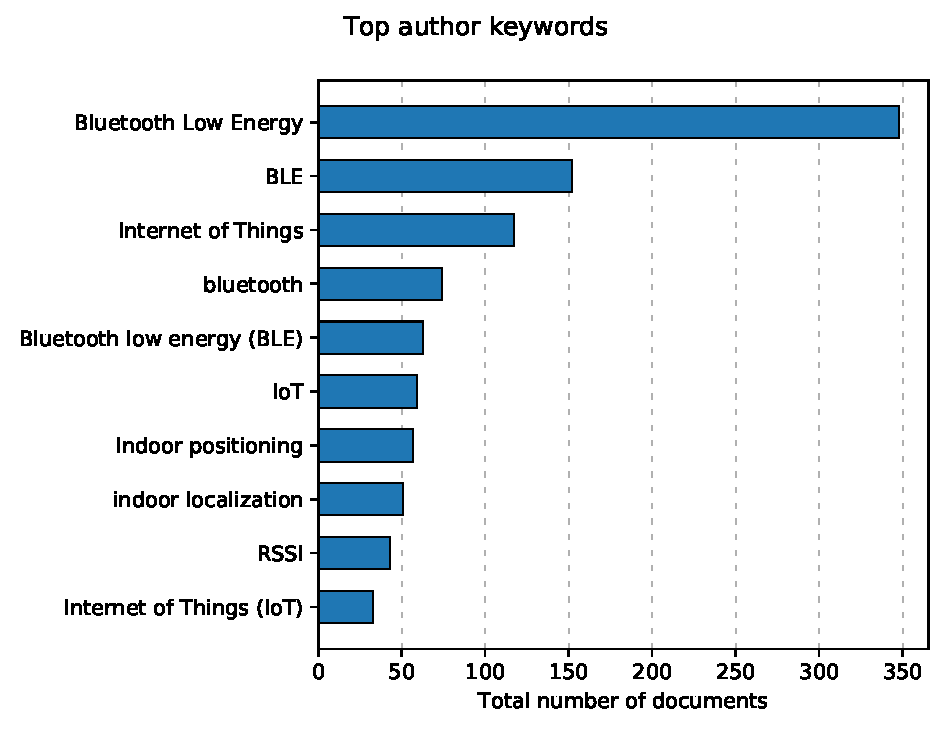
\includegraphics[width=0.5\textwidth]{./figures/graph_bar.eps}
\end{center}

\subsection{Parametric graph}
Command: 
\begin{verbatim}
python3 scientoPy.py authorKeywords --startYear 2010 --endYear 2016 --parametric \
--graphTitle "Internet of things top author keywords"
\end{verbatim}

\begin{center}
	\includegraphics[width=0.75\textwidth]{./figures/graph_parametric.eps}
\end{center}

\subsection{Parametric2 graph}
Command: 
\begin{verbatim}
python3 scientoPy.py authorKeywords --startYear 2010 --endYear 2016 --parametric2 \
--graphTitle "Internet of things top author keywords"
\end{verbatim}

\begin{center}
	\includegraphics[width=0.75\textwidth]{./figures/graph_parametric2.eps}
\end{center}


\subsection{Word cloud graph}
Command: 
\begin{verbatim}
python3 scientoPy.py authorKeywords --startYear 2010 --endYear 2016 -l 500 --wordCloud
\end{verbatim}

\begin{center}
	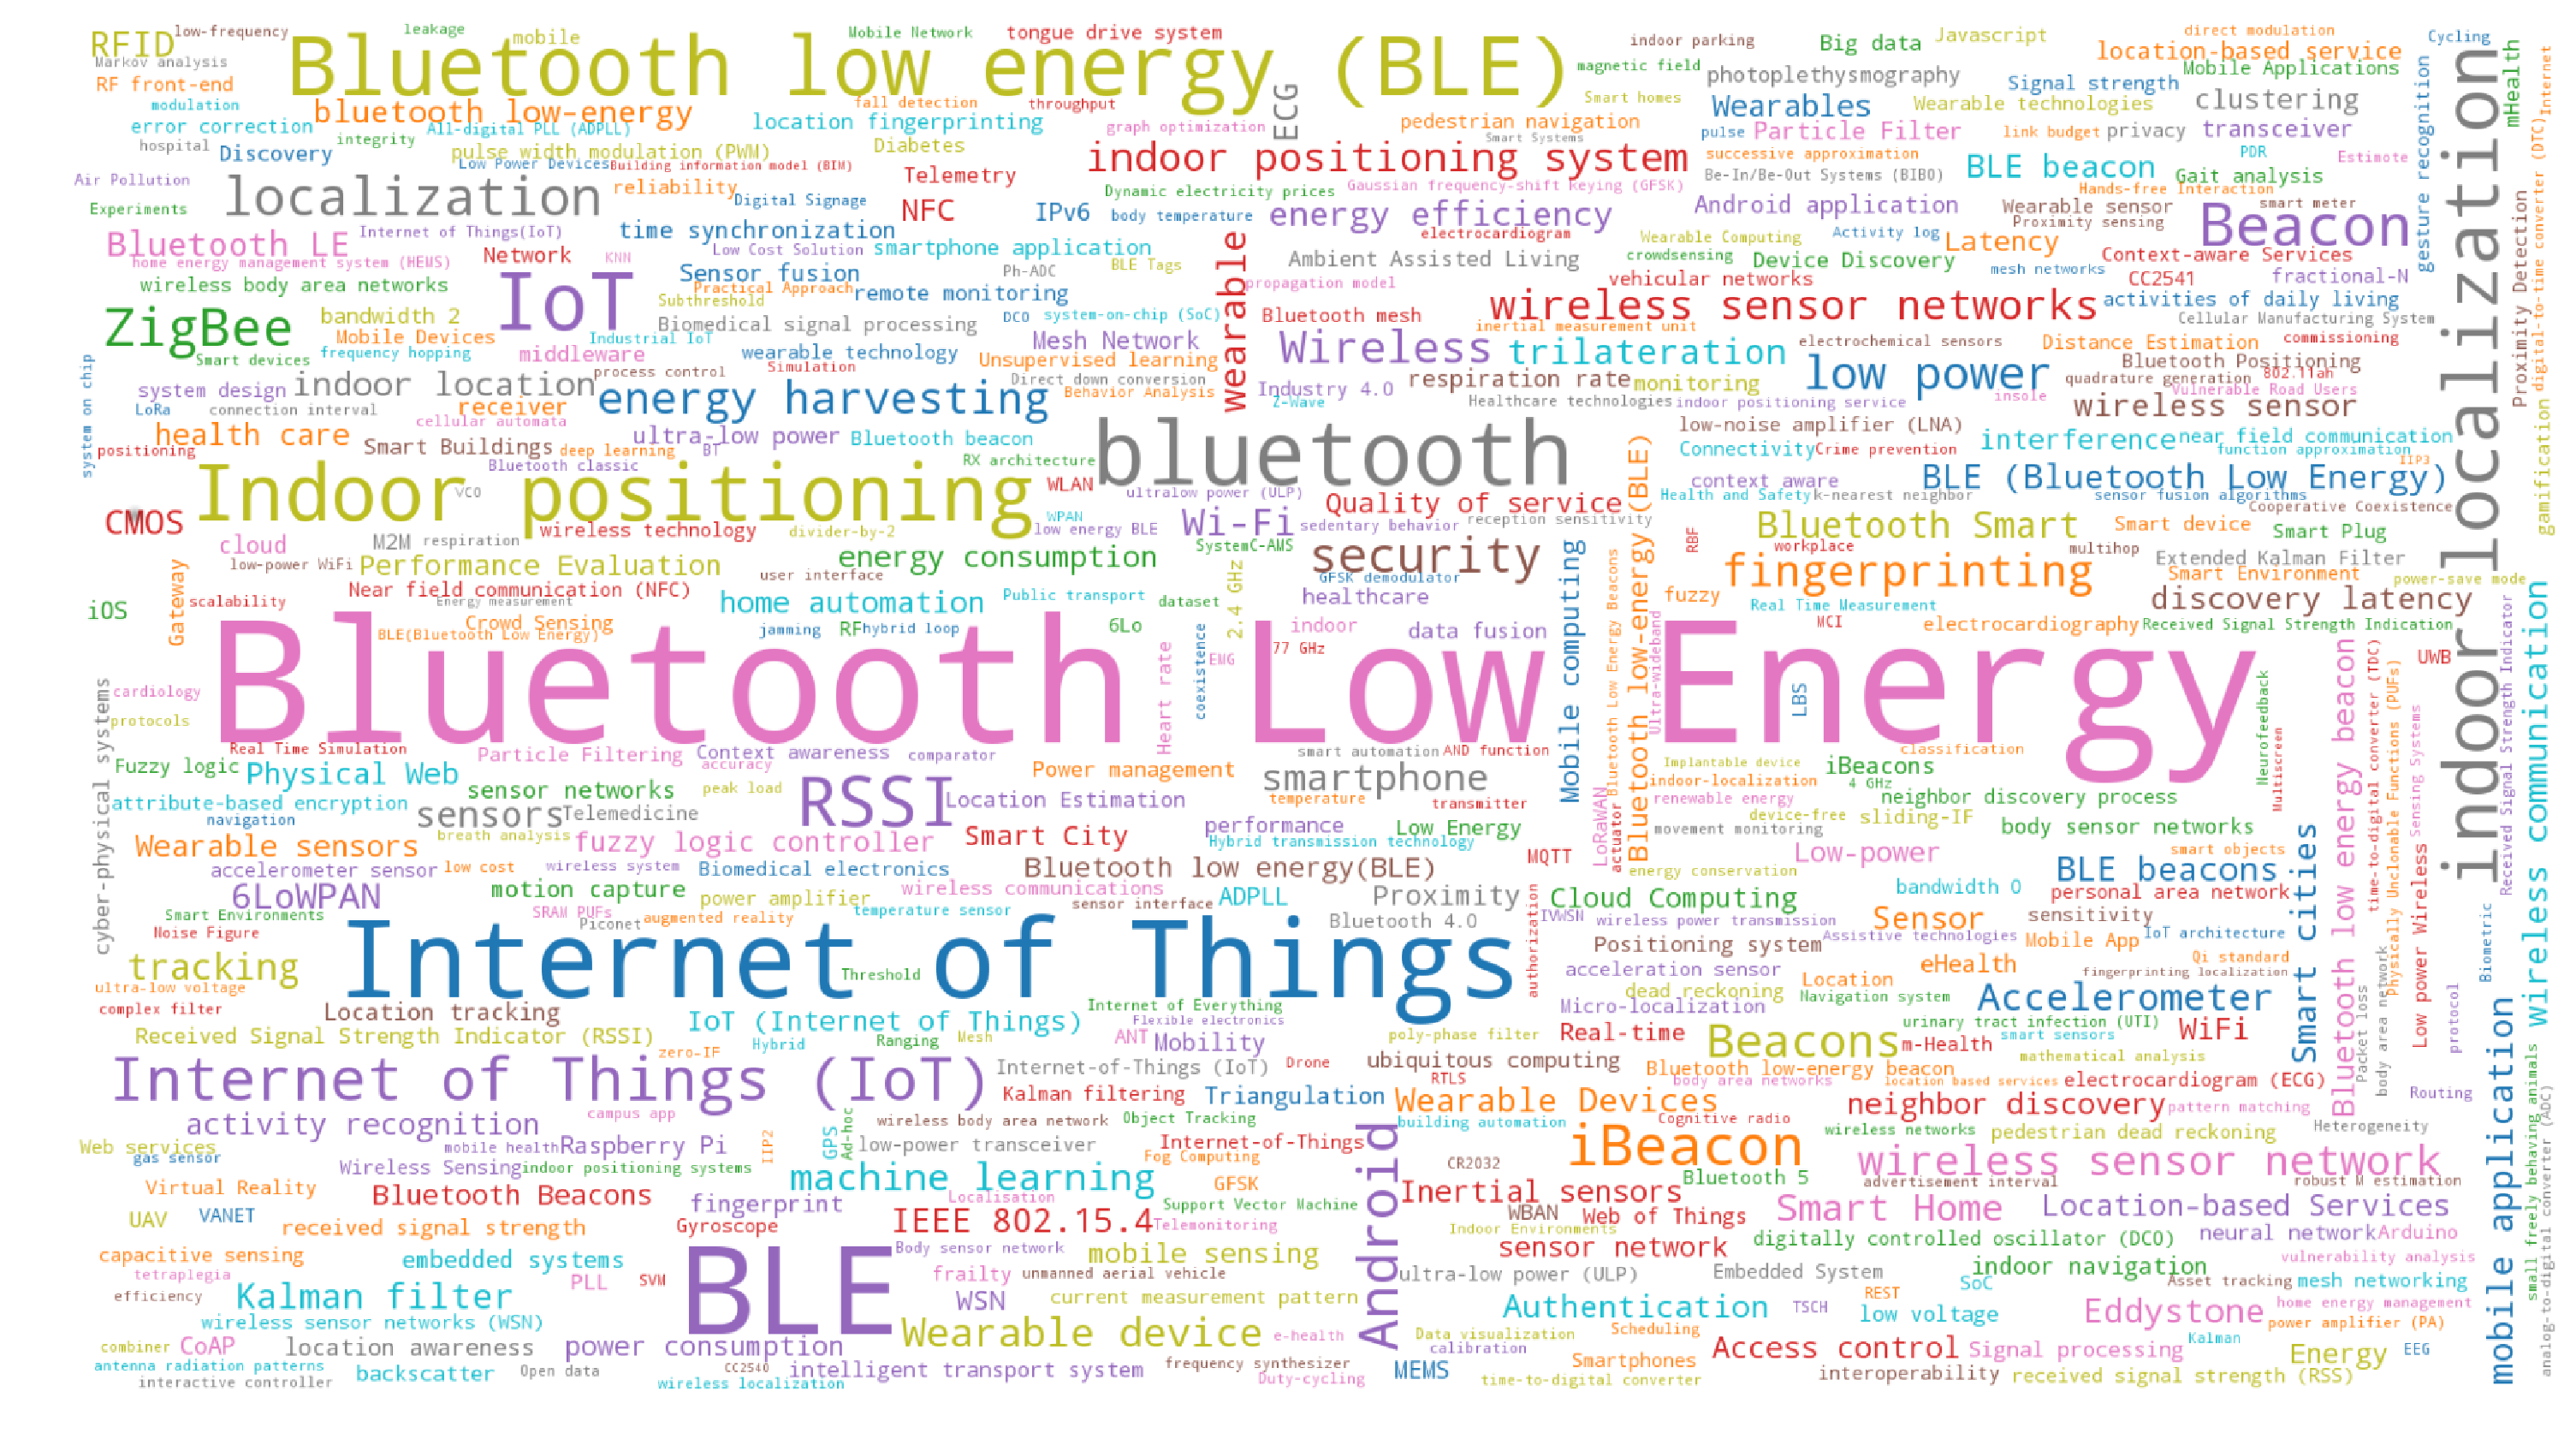
\includegraphics[width=0.75\textwidth]{./figures/graph_word_cloud.eps}
\end{center}


\end{document}  
